%%% ---------- BEGIN PASTE ----------
\begin{figure}[htbp]
\centering
\resizebox{\textwidth}{!}{%
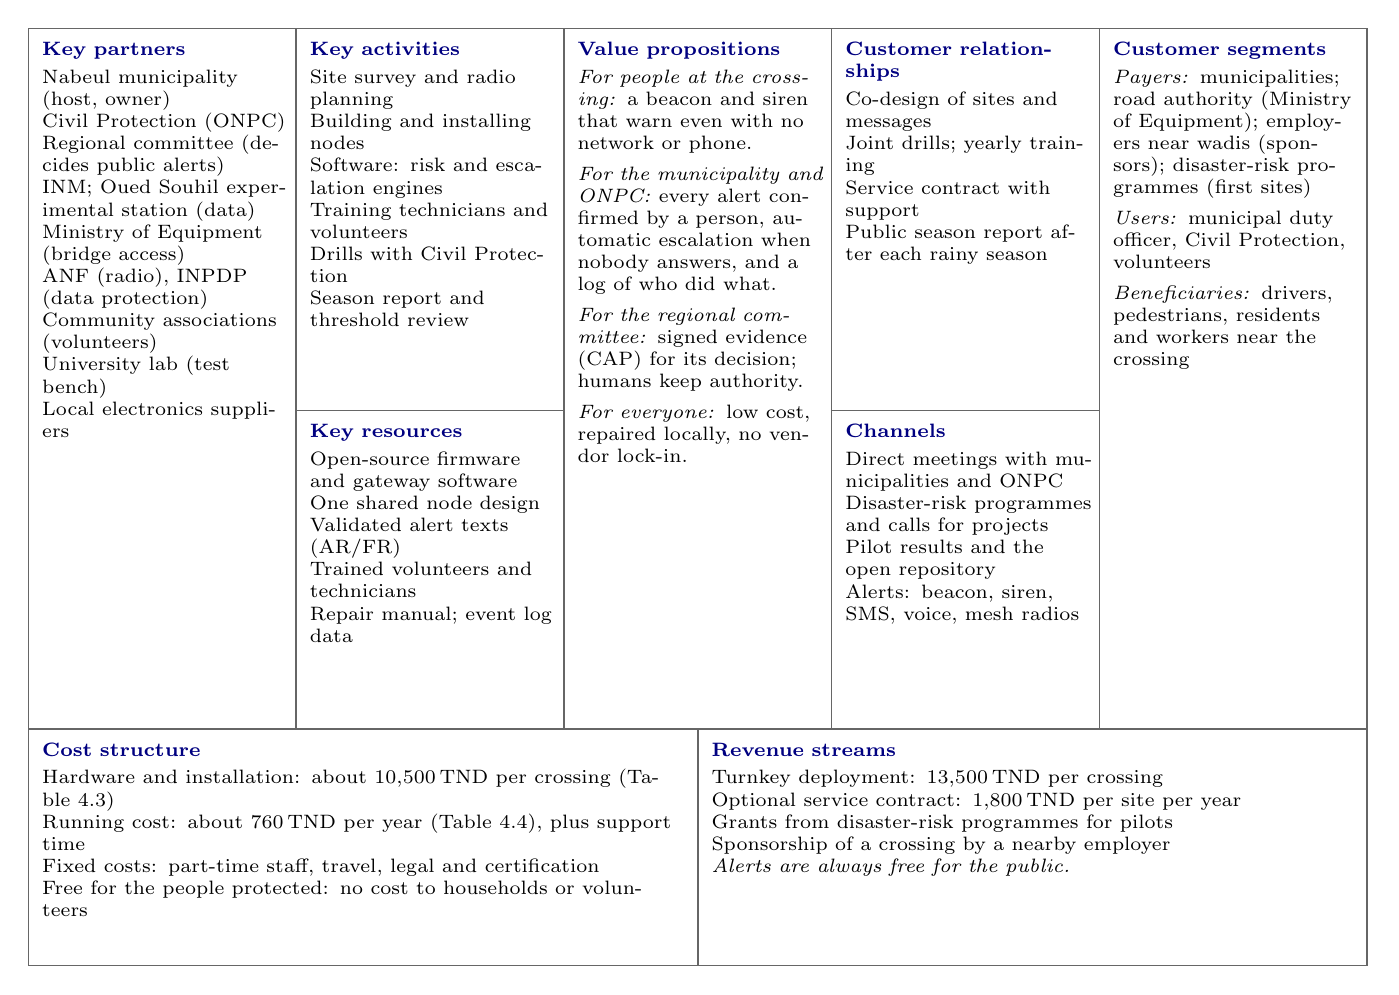
\begin{tikzpicture}[
  blk/.style={draw=black!60, line width=0.6pt, anchor=north west, inner sep=4pt,
              align=left, font=\scriptsize, text width=#1},
  ttl/.style={font=\scriptsize\bfseries, text=blue!50!black}]
  % column x positions and widths (cm): 5 columns of 3.4 cm
  \def\W{3.4}\def\H{8.9}\def\h{4.85}
  % ---- top row frames ----
  \draw[black!60, line width=0.6pt] (0,0) rectangle (5*\W,-\H);
  \foreach \i in {1,2,3,4} \draw[black!60, line width=0.6pt] (\i*\W,0) -- (\i*\W,-\H);
  \draw[black!60, line width=0.6pt] (\W,-\h) -- (2*\W,-\h);
  \draw[black!60, line width=0.6pt] (3*\W,-\h) -- (4*\W,-\h);
  % ---- bottom row frames ----
  \draw[black!60, line width=0.6pt] (0,-\H) rectangle (2.5*\W,-\H-3.0);
  \draw[black!60, line width=0.6pt] (2.5*\W,-\H) rectangle (5*\W,-\H-3.0);
  % ---- contents ----
  \node[anchor=north west, text width=3.15cm, font=\scriptsize, align=left] at (0.05,-0.05) {%
    \textbf{\textcolor{blue!50!black}{Key partners}}\\[2pt]
    Nabeul municipality (host, owner)\\
    Civil Protection (ONPC)\\
    Regional committee (decides public alerts)\\
    INM; Oued Souhil experimental station (data)\\
    Ministry of Equipment (bridge access)\\
    ANF (radio), INPDP (data protection)\\
    Community associations (volunteers)\\
    University lab (test bench)\\
    Local electronics suppliers};
  \node[anchor=north west, text width=3.15cm, font=\scriptsize, align=left] at (\W+0.05,-0.05) {%
    \textbf{\textcolor{blue!50!black}{Key activities}}\\[2pt]
    Site survey and radio planning\\
    Building and installing nodes\\
    Software: risk and escalation engines\\
    Training technicians and volunteers\\
    Drills with Civil Protection\\
    Season report and threshold review};
  \node[anchor=north west, text width=3.15cm, font=\scriptsize, align=left] at (\W+0.05,-\h-0.05) {%
    \textbf{\textcolor{blue!50!black}{Key resources}}\\[2pt]
    Open-source firmware and gateway software\\
    One shared node design\\
    Validated alert texts (AR/FR)\\
    Trained volunteers and technicians\\
    Repair manual; event log data};
  \node[anchor=north west, text width=3.15cm, font=\scriptsize, align=left] at (2*\W+0.05,-0.05) {%
    \textbf{\textcolor{blue!50!black}{Value propositions}}\\[2pt]
    \emph{For people at the crossing:} a beacon and siren that warn even with no network or phone.\\[3pt]
    \emph{For the municipality and ONPC:} every alert confirmed by a person, automatic escalation when nobody answers, and a log of who did what.\\[3pt]
    \emph{For the regional committee:} signed evidence (CAP) for its decision; humans keep authority.\\[3pt]
    \emph{For everyone:} low cost, repaired locally, no vendor lock-in.};
  \node[anchor=north west, text width=3.15cm, font=\scriptsize, align=left] at (3*\W+0.05,-0.05) {%
    \textbf{\textcolor{blue!50!black}{Customer relationships}}\\[2pt]
    Co-design of sites and messages\\
    Joint drills; yearly training\\
    Service contract with support\\
    Public season report after each rainy season};
  \node[anchor=north west, text width=3.15cm, font=\scriptsize, align=left] at (3*\W+0.05,-\h-0.05) {%
    \textbf{\textcolor{blue!50!black}{Channels}}\\[2pt]
    Direct meetings with municipalities and ONPC\\
    Disaster-risk programmes and calls for projects\\
    Pilot results and the open repository\\
    Alerts: beacon, siren, SMS, voice, mesh radios};
  \node[anchor=north west, text width=3.15cm, font=\scriptsize, align=left] at (4*\W+0.05,-0.05) {%
    \textbf{\textcolor{blue!50!black}{Customer segments}}\\[2pt]
    \emph{Payers:} municipalities; road authority (Ministry of Equipment); employers near wadis (sponsors); disaster-risk programmes (first sites)\\[3pt]
    \emph{Users:} municipal duty officer, Civil Protection, volunteers\\[3pt]
    \emph{Beneficiaries:} drivers, pedestrians, residents and workers near the crossing};
  \node[anchor=north west, text width=8.1cm, font=\scriptsize, align=left] at (0.05,-\H-0.05) {%
    \textbf{\textcolor{blue!50!black}{Cost structure}}\\[2pt]
    Hardware and installation: about 10{,}500\,TND per crossing (Table~4.3)\\
    Running cost: about 760\,TND per year (Table~4.4), plus support time\\
    Fixed costs: part-time staff, travel, legal and certification\\
    Free for the people protected: no cost to households or volunteers};
  \node[anchor=north west, text width=8.1cm, font=\scriptsize, align=left] at (2.5*\W+0.05,-\H-0.05) {%
    \textbf{\textcolor{blue!50!black}{Revenue streams}}\\[2pt]
    Turnkey deployment: 13{,}500\,TND per crossing\\
    Optional service contract: 1{,}800\,TND per site per year\\
    Grants from disaster-risk programmes for pilots\\
    Sponsorship of a crossing by a nearby employer\\
    \emph{Alerts are always free for the public.}};
\end{tikzpicture}}
\caption{Business Model Canvas for NEREUS. Prices are planning assumptions (Section~4.4).}
\label{fig:bmc}
\end{figure}
%%% ---------- END PASTE ----------
